\documentclass{article}
\usepackage{graphicx,caption}
\usepackage{enumitem}
\usepackage{epstopdf,subcaption}
\usepackage{psfrag}
\usepackage{amsmath,amssymb,epsf}
\usepackage{verbatim}
\usepackage[hyphens]{url}
\usepackage{amsmath}
\usepackage{color}
\usepackage{bbm}
\usepackage{listings}
\usepackage{setspace}
\usepackage{float}
\definecolor{Code}{rgb}{0,0,0}
\definecolor{Decorators}{rgb}{0.5,0.5,0.5}
\definecolor{Numbers}{rgb}{0.5,0,0}
\definecolor{MatchingBrackets}{rgb}{0.25,0.5,0.5}
\definecolor{Keywords}{rgb}{0,0,1}
\definecolor{self}{rgb}{0,0,0}
\definecolor{Strings}{rgb}{0,0.63,0}
\definecolor{Comments}{rgb}{0,0.63,1}
\definecolor{Backquotes}{rgb}{0,0,0}
\definecolor{Classname}{rgb}{0,0,0}
\definecolor{FunctionName}{rgb}{0,0,0}
\definecolor{Operators}{rgb}{0,0,0}
\definecolor{Background}{rgb}{0.98,0.98,0.98}
\lstdefinelanguage{Python}{
numbers=left,
numberstyle=\footnotesize,
numbersep=1em,
xleftmargin=1em,
framextopmargin=2em,
framexbottommargin=2em,
showspaces=false,
showtabs=false,
showstringspaces=false,
frame=l,
tabsize=4,
% Basic
basicstyle=\ttfamily\footnotesize\setstretch{1},
backgroundcolor=\color{Background},
% Comments
commentstyle=\color{Comments}\slshape,
% Strings
stringstyle=\color{Strings},
morecomment=[s][\color{Strings}]{"""}{"""},
morecomment=[s][\color{Strings}]{'''}{'''},
% keywords
morekeywords={import,from,class,def,for,while,if,is,in,elif,else,not,and,or
,print,break,continue,return,True,False,None,access,as,,del,except,exec
,finally,global,import,lambda,pass,print,raise,try,assert},
keywordstyle={\color{Keywords}\bfseries},
% additional keywords
morekeywords={[2]@invariant},
keywordstyle={[2]\color{Decorators}\slshape},
emph={self},
emphstyle={\color{self}\slshape},
%
}

%%% Change the following flag to toggle between questions or solutions
\def\solutions{1}

\pagestyle{empty} \addtolength{\textwidth}{1.0in}
\addtolength{\textheight}{0.5in}
\addtolength{\oddsidemargin}{-0.5in}
\addtolength{\evensidemargin}{-0.5in}
\newcommand{\ruleskip}{\bigskip\hrule\bigskip}
\newcommand{\nodify}[1]{{\sc #1}}
\newcommand{\points}[1]{{\textbf{[#1 points]}}}
\newcommand{\subquestionpoints}[1]{{[#1 points]}}
\newcommand{\xsi}{x^{(i)}}
\newcommand{\zsi}{z^{(i)}}
\newenvironment{answer}{{\bf Answer:} \sf \begingroup\color{red}}{\endgroup}%

\newcommand{\bitem}{\begin{list}{$\bullet$}%
{\setlength{\itemsep}{0pt}\setlength{\topsep}{0pt}%
\setlength{\rightmargin}{0pt}}}
\newcommand{\eitem}{\end{list}}

\setlength{\parindent}{0pt} \setlength{\parskip}{0.5ex}
\setlength{\unitlength}{1cm}

\renewcommand{\Re}{{\mathbb R}}
\newcommand{\R}{\mathbb{R}}
\newcommand{\what}[1]{\widehat{#1}}

\renewcommand{\comment}[1]{}
\newcommand{\mc}[1]{\mathcal{#1}}
\newcommand{\half}{\frac{1}{2}}
\newcommand{\KL}{D_{\text{KL}}}

\begin{document}

\pagestyle{myheadings} \markboth{}{CS229 Problem Set \#3}

\ifnum\solutions=1 {
{\huge\noindent CS 229, Fall 2018\\
Problem Set \#3 Solutions: Deep Learning \& Unsupervised learning}\\\\
YOUR NAME HERE (\texttt{YOUR SUNET HERE})
} \else {\huge
\noindent CS 229, Fall 2018\\
Problem Set \#3: Deep Learning \& Unsupervised learning
} \fi

\ruleskip

{\bf Due Wednesday, Nov 14 at 11:59 pm on Gradescope.}

\medskip

\clearpage
\item \points{25} {\bf Locally weighted linear regression}

\begin{enumerate}
	\item \subquestionpoints{10} Consider a linear regression problem in which
we want to ``weight'' different training examples differently.  Specifically,
suppose we want to minimize
%
\begin{equation*}
	J(\theta) = \frac{1}{2} \sum_{i=1}^m w^{(i)}
		\left(\theta^Tx^{(i)} - y^{(i)}\right)^2.
\end{equation*}
%
In class, we worked out what happens for the case where all the weights (the
$w^{(i)}$'s) are the same. In this problem, we will generalize some of those
ideas to the weighted setting.
\begin{enumerate}
	\item \subquestionpoints{2} Show that $J(\theta)$ can also be written
    %
    \begin{equation*}
    J(\theta) = (X\theta - {y})^T W (X\theta - {y})
    \end{equation*}
    %
    for an appropriate matrix $W$, and where $X$ and ${y}$ are as
    defined in class. Clearly specify the value of each element of the matrix
    $W$.

	\item \label{item:lwr-solution} \subquestionpoints{4} If all the $w^{(i)}$'s
    equal 1, then we saw in class that the normal equation is
    %
    \begin{equation*}
    X^TX\theta = X^T{y},
    \end{equation*}
    %
	and that the value of $\theta$ that minimizes $J(\theta)$ is given by
	$(X^TX)^{-1}X^T{y}.$
	By finding the derivative $\nabla_\theta J(\theta)$ and setting that to zero,
	generalize
	the normal equation to this weighted setting, and give the new value of
	$\theta$ that minimizes
    $J(\theta)$ in closed form as a function of $X$, $W$ and ${y}$.

	\item \subquestionpoints{4} Suppose we have a dataset
	$\{(x^{(i)}, y^{(i)});\, i=1\ldots,m\}$ of $m$ independent examples, but
    we model the $y^{(i)}$'s as drawn from conditional distributions with
    different levels of variance $(\sigma^{(i)})^2$. Specifically, assume the
    model
    %
    \begin{equation*}
		p(y^{(i)} | x^{(i)} ; \theta) = \frac{1}{\sqrt{2\pi}\sigma^{(i)}} \exp\left(-
		\frac{(y^{(i)} - \theta^Tx^{(i)})^2}{2(\sigma^{(i)})^2}\right)
	\end{equation*}
    %
    That is, each $y^{(i)}$ is drawn from a Gaussian distribution with mean
    $\theta^Tx^{(i)}$ and variance $(\sigma^{(i)})^2$ (where the
    $\sigma^{(i)}$'s are fixed, known, constants). Show that finding the
    maximum likelihood estimate of $\theta$ reduces to solving a weighted
	linear regression problem.  State clearly what the $w^{(i)}$'s are in terms of
    the $\sigma^{(i)}$'s.
\end{enumerate}

\ifnum\solutions=1
  \begin{answer}
    \begin{enumerate}
    \item
    We have

    $$
    \begin{aligned}
J(\theta) &= \sum_{i=1}^m (\theta^Tx^{(i)} - y^{(i)})(\frac{1}{2}w^{(i)}) (\theta^Tx^{(i)} - y^{(i)})\\
&= \sum_{i=1}^m (X\theta -y)^T_i (\frac{1}{2}w^{(i)}) (X\theta- y)_i
\end{aligned}
$$

If we let 

$$
W_{ij} = \begin{cases}
\frac{1}{2}w^{(i)} &i=j\\
0&\text{otherwise}
\end{cases}
$$

Then 

$$
\begin{aligned}
J(\theta)
&= \sum_{i=1}^m (X\theta -y)^T_i (\frac{1}{2}w^{(i)}) (X\theta- y)_i\\
&= \sum_{i, j=1}^m (X\theta -y)^T_i W_{ij} (X\theta- y)_j\\\\
&= (X\theta - y)^T W(X\theta - y)
\end{aligned}
$$
\item
    We have

    $$
    \begin{aligned}
\frac{\partial}{\partial \theta}J(\theta) &= \frac{\partial}{\partial \theta} (\theta^TX^TWX\theta - 2y^TW X\theta + y^TWy)\\
&=  2X^TWX\theta - 2 X^TW^Ty
\end{aligned}
$$

Taking the derivatives to zero, we find

$$
\theta = (X^TWX)^{-1}X^TW y
$$

\item

The log likelihood

$$
\begin{aligned}
l(\theta) &= \sum_{i=1}^m \log p(y^{(i)}|x^{(i)};\theta)\\
&= \sum_{i=1}^m(-\log \sqrt2\pi - \log \sigma^{(i)} - \frac{1}{2(\sigma^{(i)})^2} (y^{(i)} - \theta^Tx^{(i)})^2)
\end{aligned}
$$

Maximizing this is equivalent to minimizing

$$
            J(\theta) = \sum_{i=1}^m\frac{1}{2(\sigma^{(i)})^2} (y^{(i)} - \theta^Tx^{(i)})^2)
            $$

    \end{enumerate}

So here $w^{(i)} = 1/ (\sigma^{(i)})^2$

\end{answer}

\fi

	\clearpage
\item \subquestionpoints{10} \textbf{Coding problem.}
We will now consider the following dataset (the
formatting matches that of Datasets 1-4, except $x^{(i)}$ is 1-dimensional):
\begin{center}
	\url{data/ds5_{train,valid,test}.csv}	
\end{center}
In \texttt{src/p05b\_lwr.py}, implement locally weighted linear regression
using the normal equations you derived in Part (a) and using
%
\begin{equation*}
	w^{(i)} = \exp\left(-\frac{\|x^{(i)} - x\|_2^2}{2\tau^2}\right).
\end{equation*}
%
Train your model on the \texttt{train} split using $\tau = 0.5$, then run your
model on the \texttt{valid} split and report the mean squared error (MSE).
Finally plot your model's predictions on the validation set (plot the
training set with blue `x' markers and the validation set with a red `o'
markers). Does the model seem to be under- or overfitting?

\ifnum\solutions=1 {
  \begin{answer}
\end{answer}

} \fi

	\clearpage
\item \subquestionpoints{5} \textbf{Coding problem.}
We will now tune the hyperparameter $\tau$.
In \texttt{src/p05c\_tau.py}, find the MSE value of your model on the 
validation set for each of the values of $\tau$ specified in the code. For each
$\tau$, plot your model's predictions on the validation set in the format
described in part (b). Report the value of $\tau$ which achieves the lowest MSE
on the \texttt{valid} split, and finally report the MSE on the \texttt{test}
split using this $\tau$-value.

\ifnum\solutions=1 {
  \begin{answer}
\begin{figure}[htbp]
    \begin{subfigure}[b]{0.5\linewidth}
        \centering
        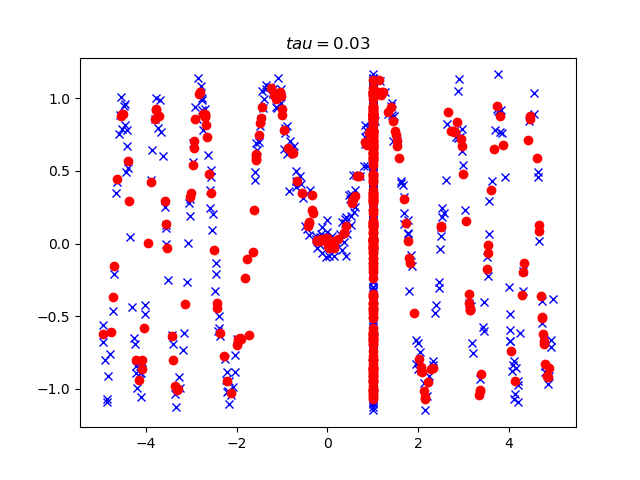
\includegraphics[width=\linewidth]{pics/tau_0d03}
    \end{subfigure}
    \begin{subfigure}[b]{0.5\linewidth}
        \centering
        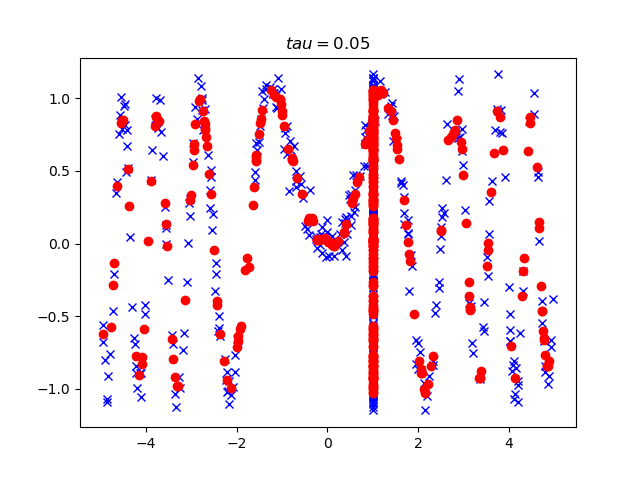
\includegraphics[width=\linewidth]{pics/tau_0d05}
    \end{subfigure}
    \begin{subfigure}[b]{0.5\linewidth}
        \centering
        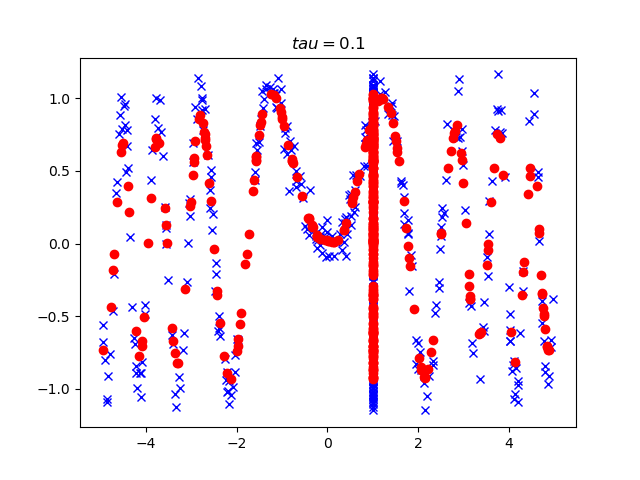
\includegraphics[width=\linewidth]{pics/tau_0d1}
    \end{subfigure}
    \begin{subfigure}[b]{0.5\linewidth}
        \centering
        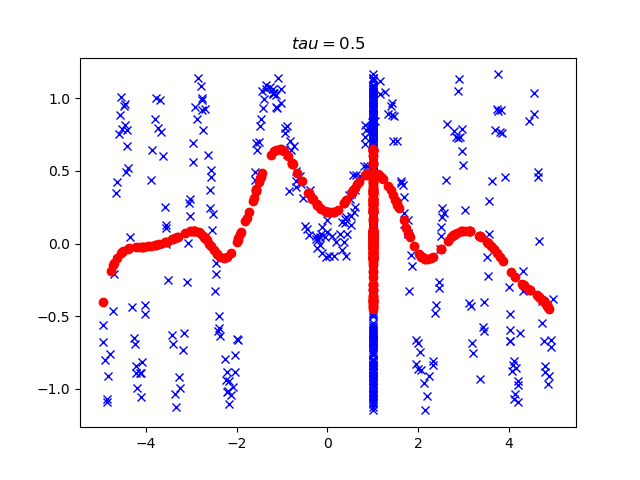
\includegraphics[width=\linewidth]{pics/tau_0d5}
    \end{subfigure}
    \begin{subfigure}[b]{0.5\linewidth}
        \centering
        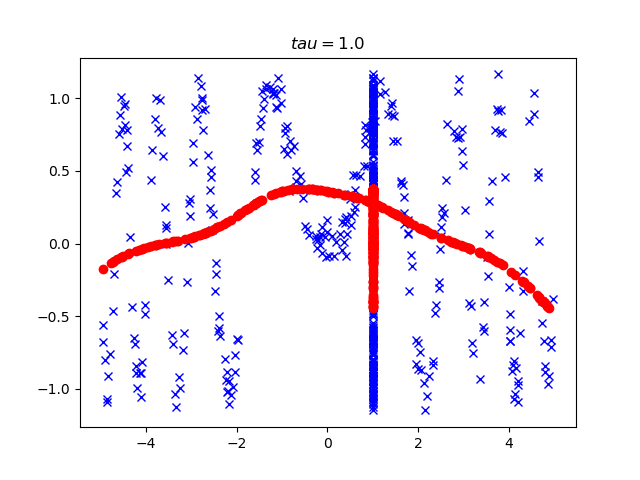
\includegraphics[width=\linewidth]{pics/tau_1d0}
    \end{subfigure}
    \begin{subfigure}[b]{0.5\linewidth}
        \centering
        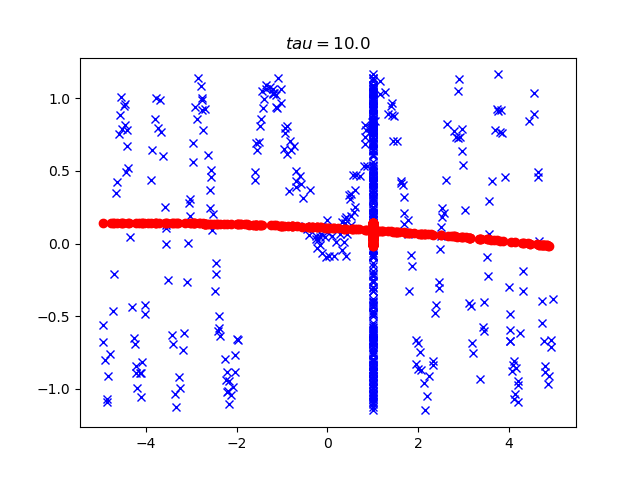
\includegraphics[width=\linewidth]{pics/tau_10d0}
    \end{subfigure}

$tau = 0.05$ achieve best result. MSE on valid set is $0.0124$, on test set is $0.0170$.

\end{figure}
\end{answer}

} \fi

\end{enumerate}


\begin{enumerate}[wide, labelwidth=!, labelindent=0pt]

\clearpage
\item \points{25} {\bf Locally weighted linear regression}

\begin{enumerate}
	\item \subquestionpoints{10} Consider a linear regression problem in which
we want to ``weight'' different training examples differently.  Specifically,
suppose we want to minimize
%
\begin{equation*}
	J(\theta) = \frac{1}{2} \sum_{i=1}^m w^{(i)}
		\left(\theta^Tx^{(i)} - y^{(i)}\right)^2.
\end{equation*}
%
In class, we worked out what happens for the case where all the weights (the
$w^{(i)}$'s) are the same. In this problem, we will generalize some of those
ideas to the weighted setting.
\begin{enumerate}
	\item \subquestionpoints{2} Show that $J(\theta)$ can also be written
    %
    \begin{equation*}
    J(\theta) = (X\theta - {y})^T W (X\theta - {y})
    \end{equation*}
    %
    for an appropriate matrix $W$, and where $X$ and ${y}$ are as
    defined in class. Clearly specify the value of each element of the matrix
    $W$.

	\item \label{item:lwr-solution} \subquestionpoints{4} If all the $w^{(i)}$'s
    equal 1, then we saw in class that the normal equation is
    %
    \begin{equation*}
    X^TX\theta = X^T{y},
    \end{equation*}
    %
	and that the value of $\theta$ that minimizes $J(\theta)$ is given by
	$(X^TX)^{-1}X^T{y}.$
	By finding the derivative $\nabla_\theta J(\theta)$ and setting that to zero,
	generalize
	the normal equation to this weighted setting, and give the new value of
	$\theta$ that minimizes
    $J(\theta)$ in closed form as a function of $X$, $W$ and ${y}$.

	\item \subquestionpoints{4} Suppose we have a dataset
	$\{(x^{(i)}, y^{(i)});\, i=1\ldots,m\}$ of $m$ independent examples, but
    we model the $y^{(i)}$'s as drawn from conditional distributions with
    different levels of variance $(\sigma^{(i)})^2$. Specifically, assume the
    model
    %
    \begin{equation*}
		p(y^{(i)} | x^{(i)} ; \theta) = \frac{1}{\sqrt{2\pi}\sigma^{(i)}} \exp\left(-
		\frac{(y^{(i)} - \theta^Tx^{(i)})^2}{2(\sigma^{(i)})^2}\right)
	\end{equation*}
    %
    That is, each $y^{(i)}$ is drawn from a Gaussian distribution with mean
    $\theta^Tx^{(i)}$ and variance $(\sigma^{(i)})^2$ (where the
    $\sigma^{(i)}$'s are fixed, known, constants). Show that finding the
    maximum likelihood estimate of $\theta$ reduces to solving a weighted
	linear regression problem.  State clearly what the $w^{(i)}$'s are in terms of
    the $\sigma^{(i)}$'s.
\end{enumerate}

\ifnum\solutions=1
  \begin{answer}
    \begin{enumerate}
    \item
    We have

    $$
    \begin{aligned}
J(\theta) &= \sum_{i=1}^m (\theta^Tx^{(i)} - y^{(i)})(\frac{1}{2}w^{(i)}) (\theta^Tx^{(i)} - y^{(i)})\\
&= \sum_{i=1}^m (X\theta -y)^T_i (\frac{1}{2}w^{(i)}) (X\theta- y)_i
\end{aligned}
$$

If we let 

$$
W_{ij} = \begin{cases}
\frac{1}{2}w^{(i)} &i=j\\
0&\text{otherwise}
\end{cases}
$$

Then 

$$
\begin{aligned}
J(\theta)
&= \sum_{i=1}^m (X\theta -y)^T_i (\frac{1}{2}w^{(i)}) (X\theta- y)_i\\
&= \sum_{i, j=1}^m (X\theta -y)^T_i W_{ij} (X\theta- y)_j\\\\
&= (X\theta - y)^T W(X\theta - y)
\end{aligned}
$$
\item
    We have

    $$
    \begin{aligned}
\frac{\partial}{\partial \theta}J(\theta) &= \frac{\partial}{\partial \theta} (\theta^TX^TWX\theta - 2y^TW X\theta + y^TWy)\\
&=  2X^TWX\theta - 2 X^TW^Ty
\end{aligned}
$$

Taking the derivatives to zero, we find

$$
\theta = (X^TWX)^{-1}X^TW y
$$

\item

The log likelihood

$$
\begin{aligned}
l(\theta) &= \sum_{i=1}^m \log p(y^{(i)}|x^{(i)};\theta)\\
&= \sum_{i=1}^m(-\log \sqrt2\pi - \log \sigma^{(i)} - \frac{1}{2(\sigma^{(i)})^2} (y^{(i)} - \theta^Tx^{(i)})^2)
\end{aligned}
$$

Maximizing this is equivalent to minimizing

$$
            J(\theta) = \sum_{i=1}^m\frac{1}{2(\sigma^{(i)})^2} (y^{(i)} - \theta^Tx^{(i)})^2)
            $$

    \end{enumerate}

So here $w^{(i)} = 1/ (\sigma^{(i)})^2$

\end{answer}

\fi

	\clearpage
\item \subquestionpoints{10} \textbf{Coding problem.}
We will now consider the following dataset (the
formatting matches that of Datasets 1-4, except $x^{(i)}$ is 1-dimensional):
\begin{center}
	\url{data/ds5_{train,valid,test}.csv}	
\end{center}
In \texttt{src/p05b\_lwr.py}, implement locally weighted linear regression
using the normal equations you derived in Part (a) and using
%
\begin{equation*}
	w^{(i)} = \exp\left(-\frac{\|x^{(i)} - x\|_2^2}{2\tau^2}\right).
\end{equation*}
%
Train your model on the \texttt{train} split using $\tau = 0.5$, then run your
model on the \texttt{valid} split and report the mean squared error (MSE).
Finally plot your model's predictions on the validation set (plot the
training set with blue `x' markers and the validation set with a red `o'
markers). Does the model seem to be under- or overfitting?

\ifnum\solutions=1 {
  \begin{answer}
\end{answer}

} \fi

	\clearpage
\item \subquestionpoints{5} \textbf{Coding problem.}
We will now tune the hyperparameter $\tau$.
In \texttt{src/p05c\_tau.py}, find the MSE value of your model on the 
validation set for each of the values of $\tau$ specified in the code. For each
$\tau$, plot your model's predictions on the validation set in the format
described in part (b). Report the value of $\tau$ which achieves the lowest MSE
on the \texttt{valid} split, and finally report the MSE on the \texttt{test}
split using this $\tau$-value.

\ifnum\solutions=1 {
  \begin{answer}
\begin{figure}[htbp]
    \begin{subfigure}[b]{0.5\linewidth}
        \centering
        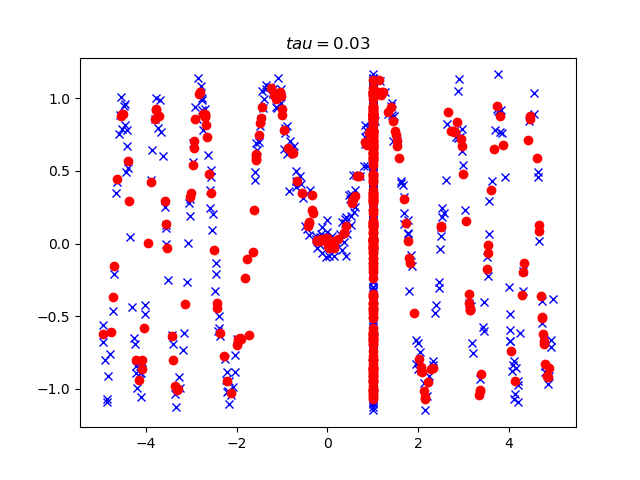
\includegraphics[width=\linewidth]{pics/tau_0d03}
    \end{subfigure}
    \begin{subfigure}[b]{0.5\linewidth}
        \centering
        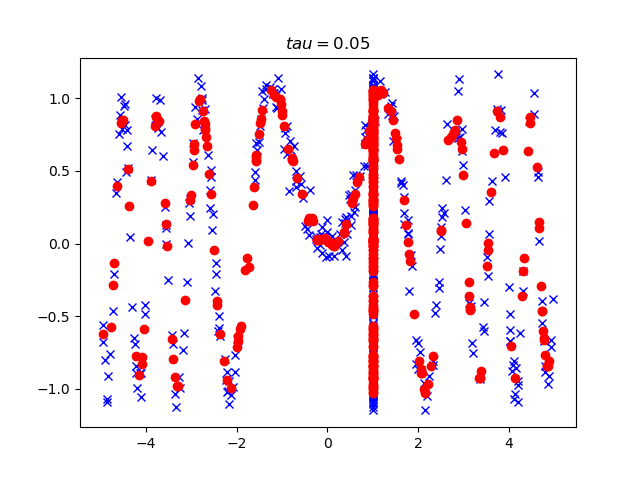
\includegraphics[width=\linewidth]{pics/tau_0d05}
    \end{subfigure}
    \begin{subfigure}[b]{0.5\linewidth}
        \centering
        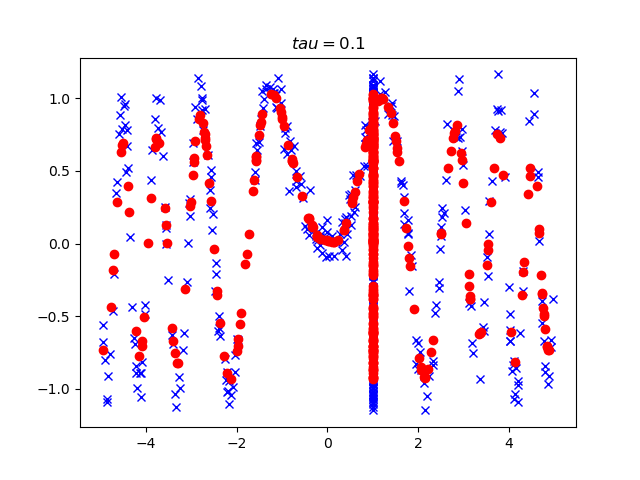
\includegraphics[width=\linewidth]{pics/tau_0d1}
    \end{subfigure}
    \begin{subfigure}[b]{0.5\linewidth}
        \centering
        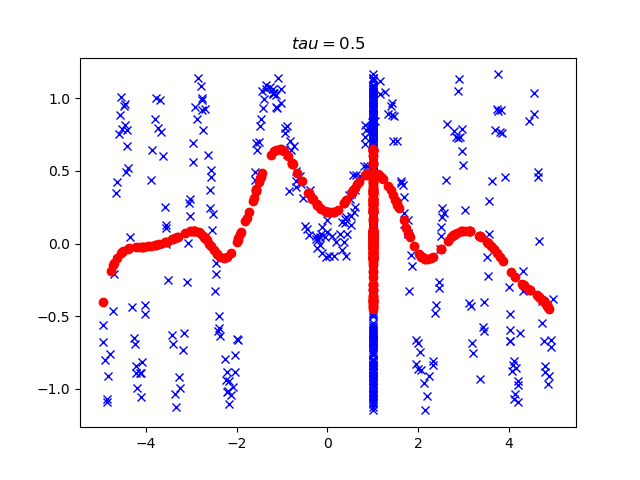
\includegraphics[width=\linewidth]{pics/tau_0d5}
    \end{subfigure}
    \begin{subfigure}[b]{0.5\linewidth}
        \centering
        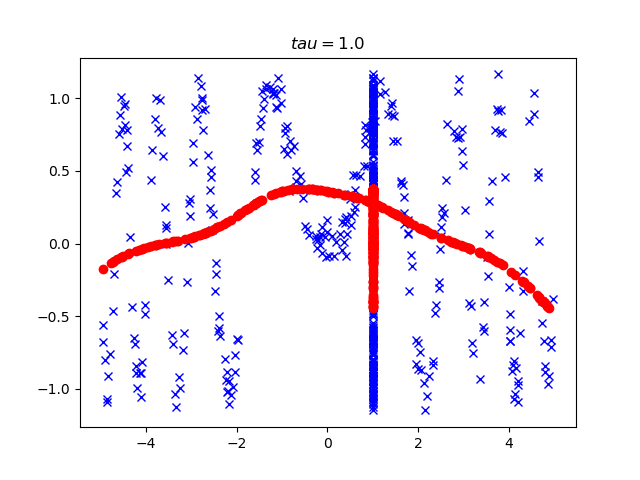
\includegraphics[width=\linewidth]{pics/tau_1d0}
    \end{subfigure}
    \begin{subfigure}[b]{0.5\linewidth}
        \centering
        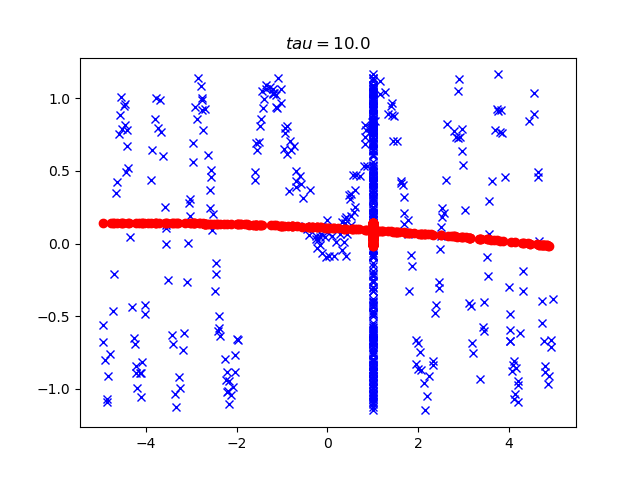
\includegraphics[width=\linewidth]{pics/tau_10d0}
    \end{subfigure}

$tau = 0.05$ achieve best result. MSE on valid set is $0.0124$, on test set is $0.0170$.

\end{figure}
\end{answer}

} \fi

\end{enumerate}


\clearpage
\item \points{25} {\bf Locally weighted linear regression}

\begin{enumerate}
	\item \subquestionpoints{10} Consider a linear regression problem in which
we want to ``weight'' different training examples differently.  Specifically,
suppose we want to minimize
%
\begin{equation*}
	J(\theta) = \frac{1}{2} \sum_{i=1}^m w^{(i)}
		\left(\theta^Tx^{(i)} - y^{(i)}\right)^2.
\end{equation*}
%
In class, we worked out what happens for the case where all the weights (the
$w^{(i)}$'s) are the same. In this problem, we will generalize some of those
ideas to the weighted setting.
\begin{enumerate}
	\item \subquestionpoints{2} Show that $J(\theta)$ can also be written
    %
    \begin{equation*}
    J(\theta) = (X\theta - {y})^T W (X\theta - {y})
    \end{equation*}
    %
    for an appropriate matrix $W$, and where $X$ and ${y}$ are as
    defined in class. Clearly specify the value of each element of the matrix
    $W$.

	\item \label{item:lwr-solution} \subquestionpoints{4} If all the $w^{(i)}$'s
    equal 1, then we saw in class that the normal equation is
    %
    \begin{equation*}
    X^TX\theta = X^T{y},
    \end{equation*}
    %
	and that the value of $\theta$ that minimizes $J(\theta)$ is given by
	$(X^TX)^{-1}X^T{y}.$
	By finding the derivative $\nabla_\theta J(\theta)$ and setting that to zero,
	generalize
	the normal equation to this weighted setting, and give the new value of
	$\theta$ that minimizes
    $J(\theta)$ in closed form as a function of $X$, $W$ and ${y}$.

	\item \subquestionpoints{4} Suppose we have a dataset
	$\{(x^{(i)}, y^{(i)});\, i=1\ldots,m\}$ of $m$ independent examples, but
    we model the $y^{(i)}$'s as drawn from conditional distributions with
    different levels of variance $(\sigma^{(i)})^2$. Specifically, assume the
    model
    %
    \begin{equation*}
		p(y^{(i)} | x^{(i)} ; \theta) = \frac{1}{\sqrt{2\pi}\sigma^{(i)}} \exp\left(-
		\frac{(y^{(i)} - \theta^Tx^{(i)})^2}{2(\sigma^{(i)})^2}\right)
	\end{equation*}
    %
    That is, each $y^{(i)}$ is drawn from a Gaussian distribution with mean
    $\theta^Tx^{(i)}$ and variance $(\sigma^{(i)})^2$ (where the
    $\sigma^{(i)}$'s are fixed, known, constants). Show that finding the
    maximum likelihood estimate of $\theta$ reduces to solving a weighted
	linear regression problem.  State clearly what the $w^{(i)}$'s are in terms of
    the $\sigma^{(i)}$'s.
\end{enumerate}

\ifnum\solutions=1
  \begin{answer}
    \begin{enumerate}
    \item
    We have

    $$
    \begin{aligned}
J(\theta) &= \sum_{i=1}^m (\theta^Tx^{(i)} - y^{(i)})(\frac{1}{2}w^{(i)}) (\theta^Tx^{(i)} - y^{(i)})\\
&= \sum_{i=1}^m (X\theta -y)^T_i (\frac{1}{2}w^{(i)}) (X\theta- y)_i
\end{aligned}
$$

If we let 

$$
W_{ij} = \begin{cases}
\frac{1}{2}w^{(i)} &i=j\\
0&\text{otherwise}
\end{cases}
$$

Then 

$$
\begin{aligned}
J(\theta)
&= \sum_{i=1}^m (X\theta -y)^T_i (\frac{1}{2}w^{(i)}) (X\theta- y)_i\\
&= \sum_{i, j=1}^m (X\theta -y)^T_i W_{ij} (X\theta- y)_j\\\\
&= (X\theta - y)^T W(X\theta - y)
\end{aligned}
$$
\item
    We have

    $$
    \begin{aligned}
\frac{\partial}{\partial \theta}J(\theta) &= \frac{\partial}{\partial \theta} (\theta^TX^TWX\theta - 2y^TW X\theta + y^TWy)\\
&=  2X^TWX\theta - 2 X^TW^Ty
\end{aligned}
$$

Taking the derivatives to zero, we find

$$
\theta = (X^TWX)^{-1}X^TW y
$$

\item

The log likelihood

$$
\begin{aligned}
l(\theta) &= \sum_{i=1}^m \log p(y^{(i)}|x^{(i)};\theta)\\
&= \sum_{i=1}^m(-\log \sqrt2\pi - \log \sigma^{(i)} - \frac{1}{2(\sigma^{(i)})^2} (y^{(i)} - \theta^Tx^{(i)})^2)
\end{aligned}
$$

Maximizing this is equivalent to minimizing

$$
            J(\theta) = \sum_{i=1}^m\frac{1}{2(\sigma^{(i)})^2} (y^{(i)} - \theta^Tx^{(i)})^2)
            $$

    \end{enumerate}

So here $w^{(i)} = 1/ (\sigma^{(i)})^2$

\end{answer}

\fi

	\clearpage
\item \subquestionpoints{10} \textbf{Coding problem.}
We will now consider the following dataset (the
formatting matches that of Datasets 1-4, except $x^{(i)}$ is 1-dimensional):
\begin{center}
	\url{data/ds5_{train,valid,test}.csv}	
\end{center}
In \texttt{src/p05b\_lwr.py}, implement locally weighted linear regression
using the normal equations you derived in Part (a) and using
%
\begin{equation*}
	w^{(i)} = \exp\left(-\frac{\|x^{(i)} - x\|_2^2}{2\tau^2}\right).
\end{equation*}
%
Train your model on the \texttt{train} split using $\tau = 0.5$, then run your
model on the \texttt{valid} split and report the mean squared error (MSE).
Finally plot your model's predictions on the validation set (plot the
training set with blue `x' markers and the validation set with a red `o'
markers). Does the model seem to be under- or overfitting?

\ifnum\solutions=1 {
  \begin{answer}
\end{answer}

} \fi

	\clearpage
\item \subquestionpoints{5} \textbf{Coding problem.}
We will now tune the hyperparameter $\tau$.
In \texttt{src/p05c\_tau.py}, find the MSE value of your model on the 
validation set for each of the values of $\tau$ specified in the code. For each
$\tau$, plot your model's predictions on the validation set in the format
described in part (b). Report the value of $\tau$ which achieves the lowest MSE
on the \texttt{valid} split, and finally report the MSE on the \texttt{test}
split using this $\tau$-value.

\ifnum\solutions=1 {
  \begin{answer}
\begin{figure}[htbp]
    \begin{subfigure}[b]{0.5\linewidth}
        \centering
        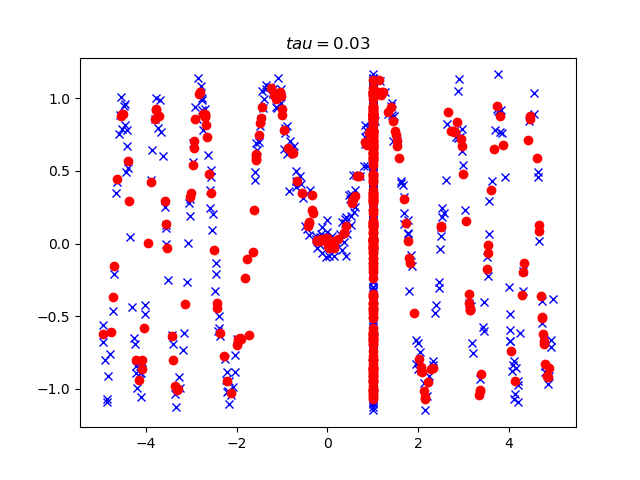
\includegraphics[width=\linewidth]{pics/tau_0d03}
    \end{subfigure}
    \begin{subfigure}[b]{0.5\linewidth}
        \centering
        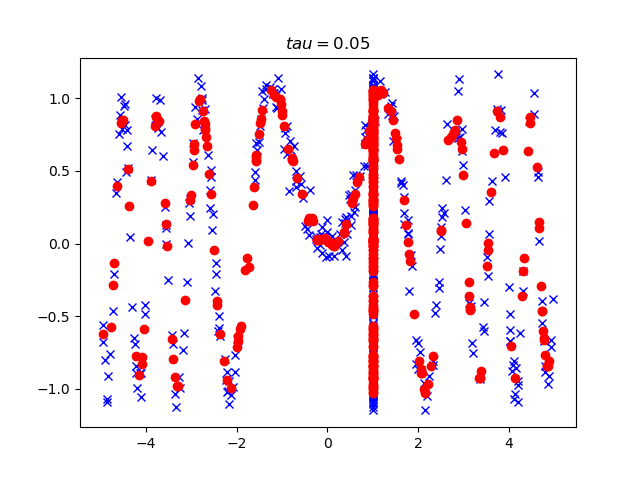
\includegraphics[width=\linewidth]{pics/tau_0d05}
    \end{subfigure}
    \begin{subfigure}[b]{0.5\linewidth}
        \centering
        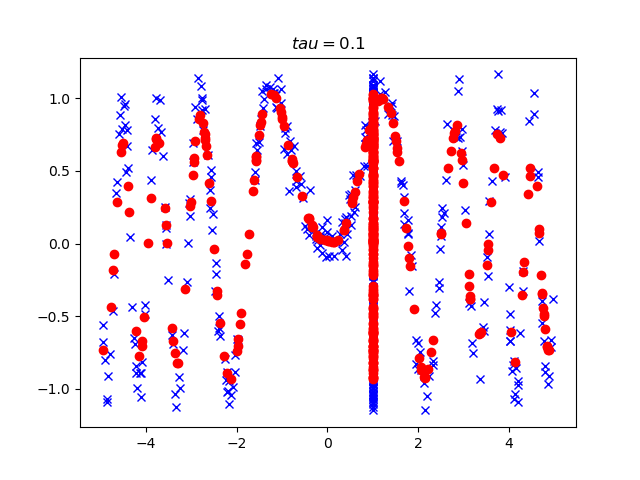
\includegraphics[width=\linewidth]{pics/tau_0d1}
    \end{subfigure}
    \begin{subfigure}[b]{0.5\linewidth}
        \centering
        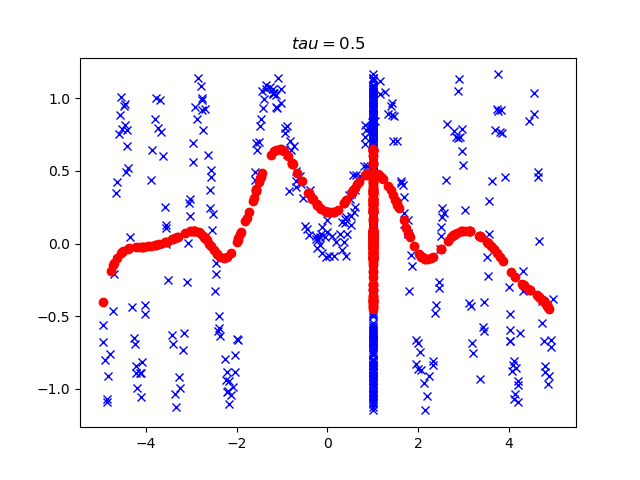
\includegraphics[width=\linewidth]{pics/tau_0d5}
    \end{subfigure}
    \begin{subfigure}[b]{0.5\linewidth}
        \centering
        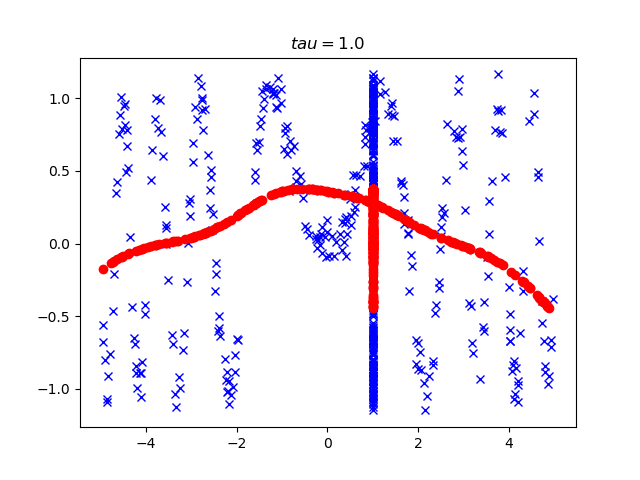
\includegraphics[width=\linewidth]{pics/tau_1d0}
    \end{subfigure}
    \begin{subfigure}[b]{0.5\linewidth}
        \centering
        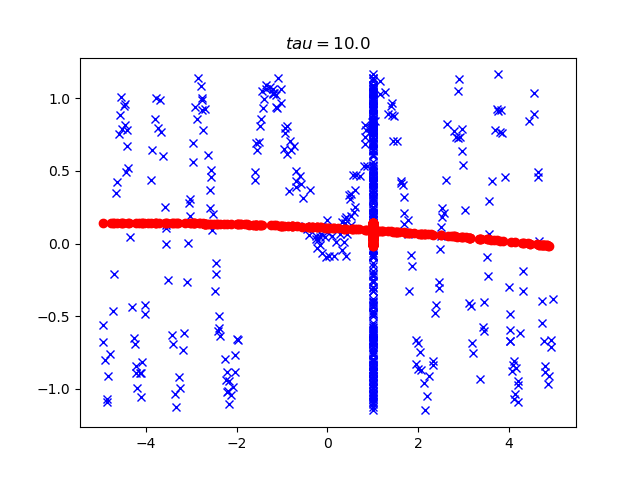
\includegraphics[width=\linewidth]{pics/tau_10d0}
    \end{subfigure}

$tau = 0.05$ achieve best result. MSE on valid set is $0.0124$, on test set is $0.0170$.

\end{figure}
\end{answer}

} \fi

\end{enumerate}


\clearpage
\item \points{25} {\bf Locally weighted linear regression}

\begin{enumerate}
	\item \subquestionpoints{10} Consider a linear regression problem in which
we want to ``weight'' different training examples differently.  Specifically,
suppose we want to minimize
%
\begin{equation*}
	J(\theta) = \frac{1}{2} \sum_{i=1}^m w^{(i)}
		\left(\theta^Tx^{(i)} - y^{(i)}\right)^2.
\end{equation*}
%
In class, we worked out what happens for the case where all the weights (the
$w^{(i)}$'s) are the same. In this problem, we will generalize some of those
ideas to the weighted setting.
\begin{enumerate}
	\item \subquestionpoints{2} Show that $J(\theta)$ can also be written
    %
    \begin{equation*}
    J(\theta) = (X\theta - {y})^T W (X\theta - {y})
    \end{equation*}
    %
    for an appropriate matrix $W$, and where $X$ and ${y}$ are as
    defined in class. Clearly specify the value of each element of the matrix
    $W$.

	\item \label{item:lwr-solution} \subquestionpoints{4} If all the $w^{(i)}$'s
    equal 1, then we saw in class that the normal equation is
    %
    \begin{equation*}
    X^TX\theta = X^T{y},
    \end{equation*}
    %
	and that the value of $\theta$ that minimizes $J(\theta)$ is given by
	$(X^TX)^{-1}X^T{y}.$
	By finding the derivative $\nabla_\theta J(\theta)$ and setting that to zero,
	generalize
	the normal equation to this weighted setting, and give the new value of
	$\theta$ that minimizes
    $J(\theta)$ in closed form as a function of $X$, $W$ and ${y}$.

	\item \subquestionpoints{4} Suppose we have a dataset
	$\{(x^{(i)}, y^{(i)});\, i=1\ldots,m\}$ of $m$ independent examples, but
    we model the $y^{(i)}$'s as drawn from conditional distributions with
    different levels of variance $(\sigma^{(i)})^2$. Specifically, assume the
    model
    %
    \begin{equation*}
		p(y^{(i)} | x^{(i)} ; \theta) = \frac{1}{\sqrt{2\pi}\sigma^{(i)}} \exp\left(-
		\frac{(y^{(i)} - \theta^Tx^{(i)})^2}{2(\sigma^{(i)})^2}\right)
	\end{equation*}
    %
    That is, each $y^{(i)}$ is drawn from a Gaussian distribution with mean
    $\theta^Tx^{(i)}$ and variance $(\sigma^{(i)})^2$ (where the
    $\sigma^{(i)}$'s are fixed, known, constants). Show that finding the
    maximum likelihood estimate of $\theta$ reduces to solving a weighted
	linear regression problem.  State clearly what the $w^{(i)}$'s are in terms of
    the $\sigma^{(i)}$'s.
\end{enumerate}

\ifnum\solutions=1
  \begin{answer}
    \begin{enumerate}
    \item
    We have

    $$
    \begin{aligned}
J(\theta) &= \sum_{i=1}^m (\theta^Tx^{(i)} - y^{(i)})(\frac{1}{2}w^{(i)}) (\theta^Tx^{(i)} - y^{(i)})\\
&= \sum_{i=1}^m (X\theta -y)^T_i (\frac{1}{2}w^{(i)}) (X\theta- y)_i
\end{aligned}
$$

If we let 

$$
W_{ij} = \begin{cases}
\frac{1}{2}w^{(i)} &i=j\\
0&\text{otherwise}
\end{cases}
$$

Then 

$$
\begin{aligned}
J(\theta)
&= \sum_{i=1}^m (X\theta -y)^T_i (\frac{1}{2}w^{(i)}) (X\theta- y)_i\\
&= \sum_{i, j=1}^m (X\theta -y)^T_i W_{ij} (X\theta- y)_j\\\\
&= (X\theta - y)^T W(X\theta - y)
\end{aligned}
$$
\item
    We have

    $$
    \begin{aligned}
\frac{\partial}{\partial \theta}J(\theta) &= \frac{\partial}{\partial \theta} (\theta^TX^TWX\theta - 2y^TW X\theta + y^TWy)\\
&=  2X^TWX\theta - 2 X^TW^Ty
\end{aligned}
$$

Taking the derivatives to zero, we find

$$
\theta = (X^TWX)^{-1}X^TW y
$$

\item

The log likelihood

$$
\begin{aligned}
l(\theta) &= \sum_{i=1}^m \log p(y^{(i)}|x^{(i)};\theta)\\
&= \sum_{i=1}^m(-\log \sqrt2\pi - \log \sigma^{(i)} - \frac{1}{2(\sigma^{(i)})^2} (y^{(i)} - \theta^Tx^{(i)})^2)
\end{aligned}
$$

Maximizing this is equivalent to minimizing

$$
            J(\theta) = \sum_{i=1}^m\frac{1}{2(\sigma^{(i)})^2} (y^{(i)} - \theta^Tx^{(i)})^2)
            $$

    \end{enumerate}

So here $w^{(i)} = 1/ (\sigma^{(i)})^2$

\end{answer}

\fi

	\clearpage
\item \subquestionpoints{10} \textbf{Coding problem.}
We will now consider the following dataset (the
formatting matches that of Datasets 1-4, except $x^{(i)}$ is 1-dimensional):
\begin{center}
	\url{data/ds5_{train,valid,test}.csv}	
\end{center}
In \texttt{src/p05b\_lwr.py}, implement locally weighted linear regression
using the normal equations you derived in Part (a) and using
%
\begin{equation*}
	w^{(i)} = \exp\left(-\frac{\|x^{(i)} - x\|_2^2}{2\tau^2}\right).
\end{equation*}
%
Train your model on the \texttt{train} split using $\tau = 0.5$, then run your
model on the \texttt{valid} split and report the mean squared error (MSE).
Finally plot your model's predictions on the validation set (plot the
training set with blue `x' markers and the validation set with a red `o'
markers). Does the model seem to be under- or overfitting?

\ifnum\solutions=1 {
  \begin{answer}
\end{answer}

} \fi

	\clearpage
\item \subquestionpoints{5} \textbf{Coding problem.}
We will now tune the hyperparameter $\tau$.
In \texttt{src/p05c\_tau.py}, find the MSE value of your model on the 
validation set for each of the values of $\tau$ specified in the code. For each
$\tau$, plot your model's predictions on the validation set in the format
described in part (b). Report the value of $\tau$ which achieves the lowest MSE
on the \texttt{valid} split, and finally report the MSE on the \texttt{test}
split using this $\tau$-value.

\ifnum\solutions=1 {
  \begin{answer}
\begin{figure}[htbp]
    \begin{subfigure}[b]{0.5\linewidth}
        \centering
        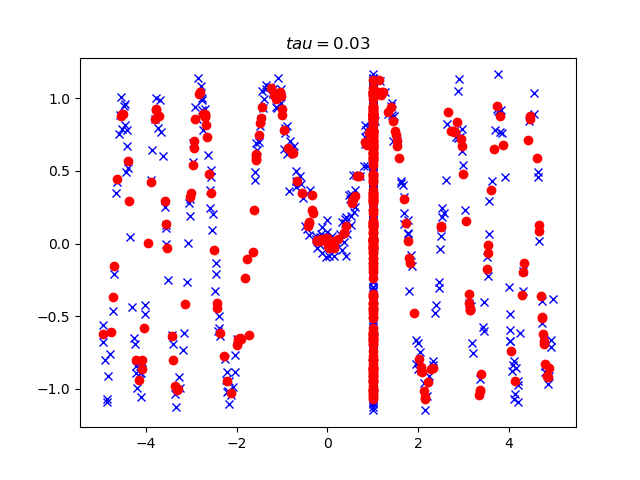
\includegraphics[width=\linewidth]{pics/tau_0d03}
    \end{subfigure}
    \begin{subfigure}[b]{0.5\linewidth}
        \centering
        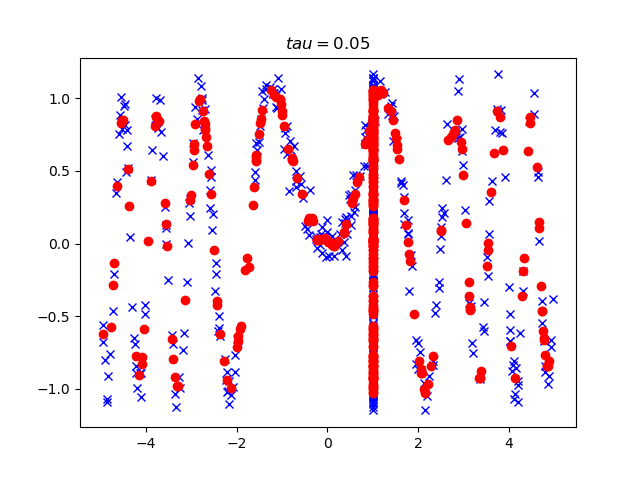
\includegraphics[width=\linewidth]{pics/tau_0d05}
    \end{subfigure}
    \begin{subfigure}[b]{0.5\linewidth}
        \centering
        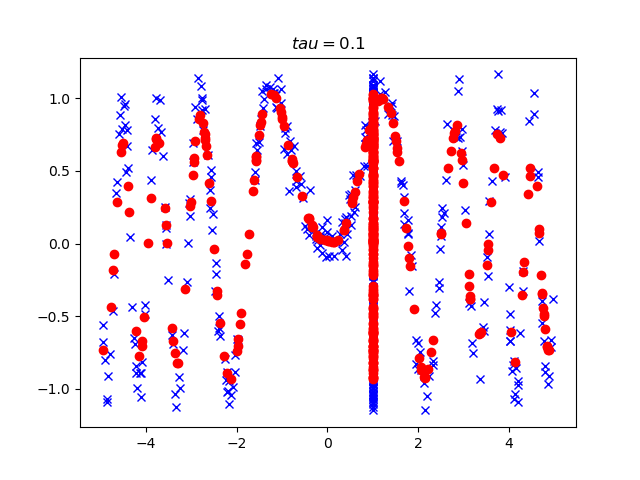
\includegraphics[width=\linewidth]{pics/tau_0d1}
    \end{subfigure}
    \begin{subfigure}[b]{0.5\linewidth}
        \centering
        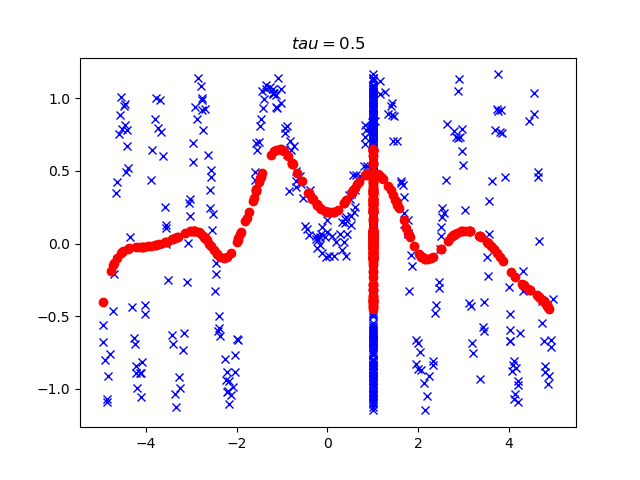
\includegraphics[width=\linewidth]{pics/tau_0d5}
    \end{subfigure}
    \begin{subfigure}[b]{0.5\linewidth}
        \centering
        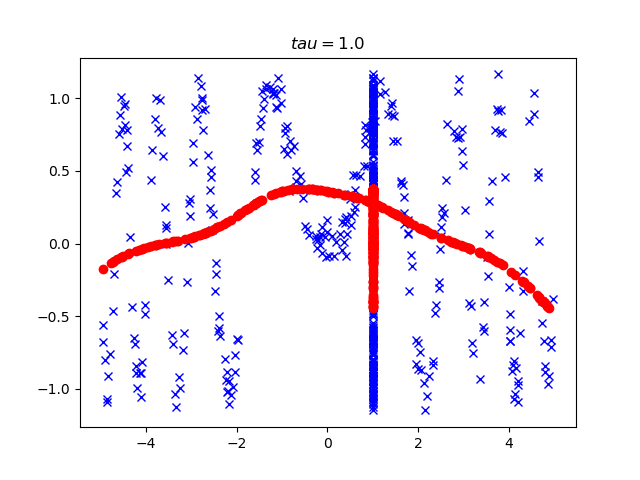
\includegraphics[width=\linewidth]{pics/tau_1d0}
    \end{subfigure}
    \begin{subfigure}[b]{0.5\linewidth}
        \centering
        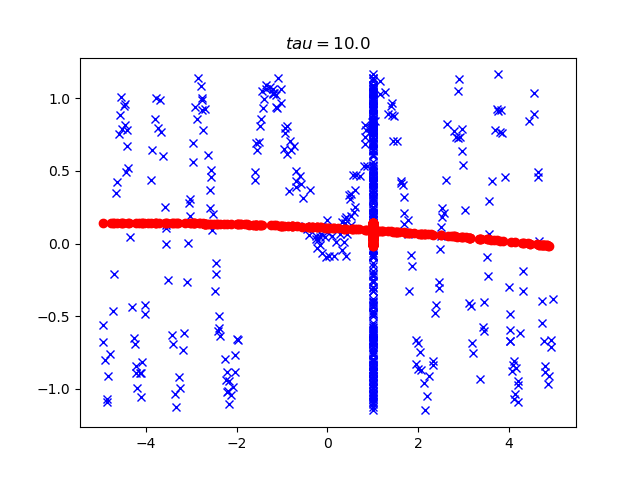
\includegraphics[width=\linewidth]{pics/tau_10d0}
    \end{subfigure}

$tau = 0.05$ achieve best result. MSE on valid set is $0.0124$, on test set is $0.0170$.

\end{figure}
\end{answer}

} \fi

\end{enumerate}


\clearpage
\item \points{25} {\bf Locally weighted linear regression}

\begin{enumerate}
	\item \subquestionpoints{10} Consider a linear regression problem in which
we want to ``weight'' different training examples differently.  Specifically,
suppose we want to minimize
%
\begin{equation*}
	J(\theta) = \frac{1}{2} \sum_{i=1}^m w^{(i)}
		\left(\theta^Tx^{(i)} - y^{(i)}\right)^2.
\end{equation*}
%
In class, we worked out what happens for the case where all the weights (the
$w^{(i)}$'s) are the same. In this problem, we will generalize some of those
ideas to the weighted setting.
\begin{enumerate}
	\item \subquestionpoints{2} Show that $J(\theta)$ can also be written
    %
    \begin{equation*}
    J(\theta) = (X\theta - {y})^T W (X\theta - {y})
    \end{equation*}
    %
    for an appropriate matrix $W$, and where $X$ and ${y}$ are as
    defined in class. Clearly specify the value of each element of the matrix
    $W$.

	\item \label{item:lwr-solution} \subquestionpoints{4} If all the $w^{(i)}$'s
    equal 1, then we saw in class that the normal equation is
    %
    \begin{equation*}
    X^TX\theta = X^T{y},
    \end{equation*}
    %
	and that the value of $\theta$ that minimizes $J(\theta)$ is given by
	$(X^TX)^{-1}X^T{y}.$
	By finding the derivative $\nabla_\theta J(\theta)$ and setting that to zero,
	generalize
	the normal equation to this weighted setting, and give the new value of
	$\theta$ that minimizes
    $J(\theta)$ in closed form as a function of $X$, $W$ and ${y}$.

	\item \subquestionpoints{4} Suppose we have a dataset
	$\{(x^{(i)}, y^{(i)});\, i=1\ldots,m\}$ of $m$ independent examples, but
    we model the $y^{(i)}$'s as drawn from conditional distributions with
    different levels of variance $(\sigma^{(i)})^2$. Specifically, assume the
    model
    %
    \begin{equation*}
		p(y^{(i)} | x^{(i)} ; \theta) = \frac{1}{\sqrt{2\pi}\sigma^{(i)}} \exp\left(-
		\frac{(y^{(i)} - \theta^Tx^{(i)})^2}{2(\sigma^{(i)})^2}\right)
	\end{equation*}
    %
    That is, each $y^{(i)}$ is drawn from a Gaussian distribution with mean
    $\theta^Tx^{(i)}$ and variance $(\sigma^{(i)})^2$ (where the
    $\sigma^{(i)}$'s are fixed, known, constants). Show that finding the
    maximum likelihood estimate of $\theta$ reduces to solving a weighted
	linear regression problem.  State clearly what the $w^{(i)}$'s are in terms of
    the $\sigma^{(i)}$'s.
\end{enumerate}

\ifnum\solutions=1
  \begin{answer}
    \begin{enumerate}
    \item
    We have

    $$
    \begin{aligned}
J(\theta) &= \sum_{i=1}^m (\theta^Tx^{(i)} - y^{(i)})(\frac{1}{2}w^{(i)}) (\theta^Tx^{(i)} - y^{(i)})\\
&= \sum_{i=1}^m (X\theta -y)^T_i (\frac{1}{2}w^{(i)}) (X\theta- y)_i
\end{aligned}
$$

If we let 

$$
W_{ij} = \begin{cases}
\frac{1}{2}w^{(i)} &i=j\\
0&\text{otherwise}
\end{cases}
$$

Then 

$$
\begin{aligned}
J(\theta)
&= \sum_{i=1}^m (X\theta -y)^T_i (\frac{1}{2}w^{(i)}) (X\theta- y)_i\\
&= \sum_{i, j=1}^m (X\theta -y)^T_i W_{ij} (X\theta- y)_j\\\\
&= (X\theta - y)^T W(X\theta - y)
\end{aligned}
$$
\item
    We have

    $$
    \begin{aligned}
\frac{\partial}{\partial \theta}J(\theta) &= \frac{\partial}{\partial \theta} (\theta^TX^TWX\theta - 2y^TW X\theta + y^TWy)\\
&=  2X^TWX\theta - 2 X^TW^Ty
\end{aligned}
$$

Taking the derivatives to zero, we find

$$
\theta = (X^TWX)^{-1}X^TW y
$$

\item

The log likelihood

$$
\begin{aligned}
l(\theta) &= \sum_{i=1}^m \log p(y^{(i)}|x^{(i)};\theta)\\
&= \sum_{i=1}^m(-\log \sqrt2\pi - \log \sigma^{(i)} - \frac{1}{2(\sigma^{(i)})^2} (y^{(i)} - \theta^Tx^{(i)})^2)
\end{aligned}
$$

Maximizing this is equivalent to minimizing

$$
            J(\theta) = \sum_{i=1}^m\frac{1}{2(\sigma^{(i)})^2} (y^{(i)} - \theta^Tx^{(i)})^2)
            $$

    \end{enumerate}

So here $w^{(i)} = 1/ (\sigma^{(i)})^2$

\end{answer}

\fi

	\clearpage
\item \subquestionpoints{10} \textbf{Coding problem.}
We will now consider the following dataset (the
formatting matches that of Datasets 1-4, except $x^{(i)}$ is 1-dimensional):
\begin{center}
	\url{data/ds5_{train,valid,test}.csv}	
\end{center}
In \texttt{src/p05b\_lwr.py}, implement locally weighted linear regression
using the normal equations you derived in Part (a) and using
%
\begin{equation*}
	w^{(i)} = \exp\left(-\frac{\|x^{(i)} - x\|_2^2}{2\tau^2}\right).
\end{equation*}
%
Train your model on the \texttt{train} split using $\tau = 0.5$, then run your
model on the \texttt{valid} split and report the mean squared error (MSE).
Finally plot your model's predictions on the validation set (plot the
training set with blue `x' markers and the validation set with a red `o'
markers). Does the model seem to be under- or overfitting?

\ifnum\solutions=1 {
  \begin{answer}
\end{answer}

} \fi

	\clearpage
\item \subquestionpoints{5} \textbf{Coding problem.}
We will now tune the hyperparameter $\tau$.
In \texttt{src/p05c\_tau.py}, find the MSE value of your model on the 
validation set for each of the values of $\tau$ specified in the code. For each
$\tau$, plot your model's predictions on the validation set in the format
described in part (b). Report the value of $\tau$ which achieves the lowest MSE
on the \texttt{valid} split, and finally report the MSE on the \texttt{test}
split using this $\tau$-value.

\ifnum\solutions=1 {
  \begin{answer}
\begin{figure}[htbp]
    \begin{subfigure}[b]{0.5\linewidth}
        \centering
        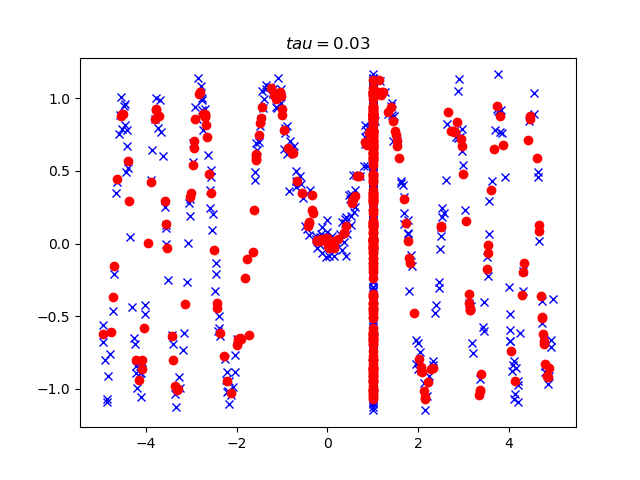
\includegraphics[width=\linewidth]{pics/tau_0d03}
    \end{subfigure}
    \begin{subfigure}[b]{0.5\linewidth}
        \centering
        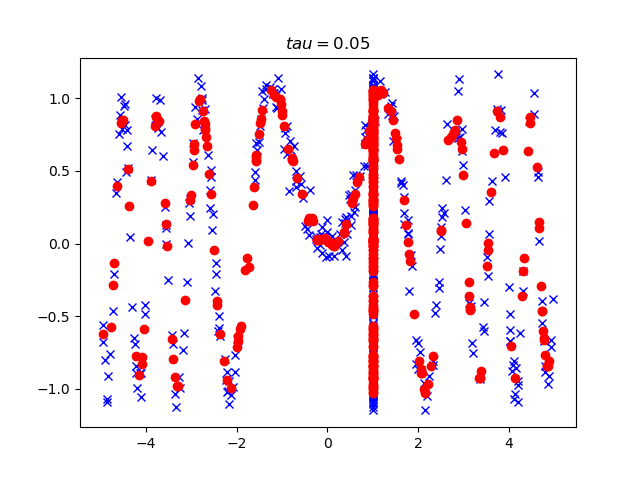
\includegraphics[width=\linewidth]{pics/tau_0d05}
    \end{subfigure}
    \begin{subfigure}[b]{0.5\linewidth}
        \centering
        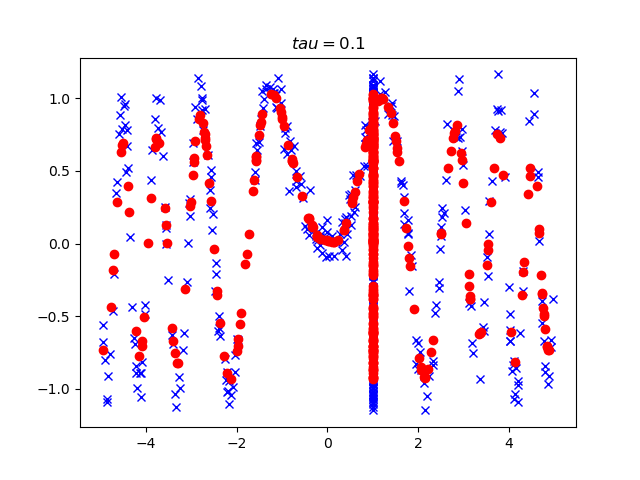
\includegraphics[width=\linewidth]{pics/tau_0d1}
    \end{subfigure}
    \begin{subfigure}[b]{0.5\linewidth}
        \centering
        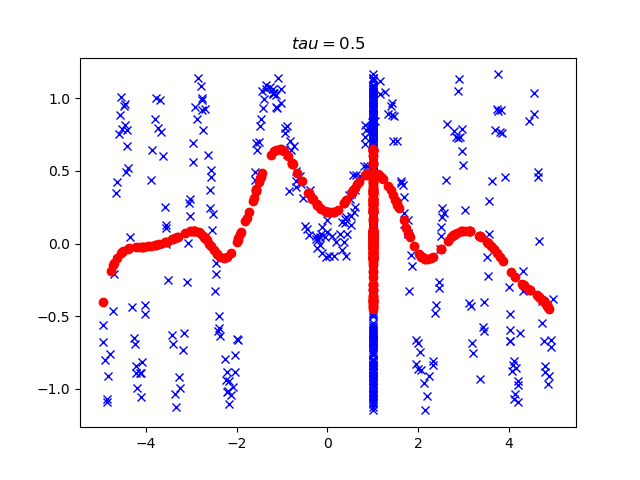
\includegraphics[width=\linewidth]{pics/tau_0d5}
    \end{subfigure}
    \begin{subfigure}[b]{0.5\linewidth}
        \centering
        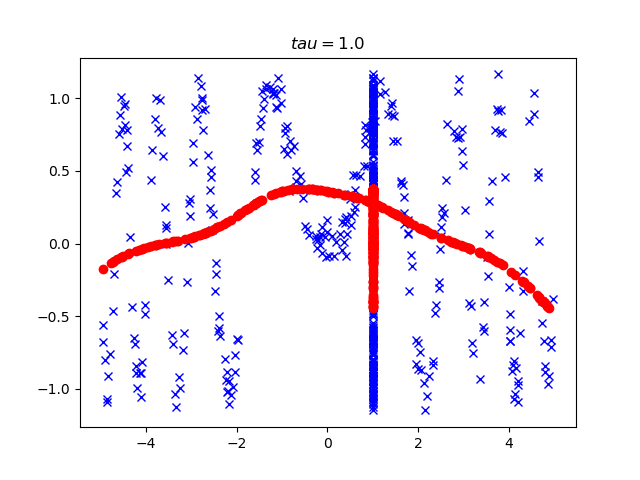
\includegraphics[width=\linewidth]{pics/tau_1d0}
    \end{subfigure}
    \begin{subfigure}[b]{0.5\linewidth}
        \centering
        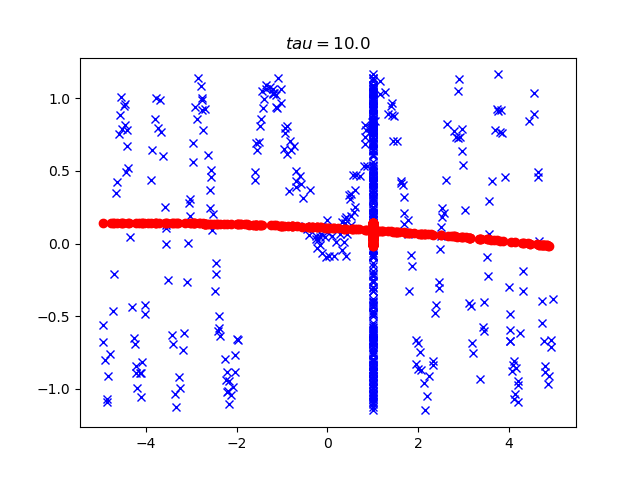
\includegraphics[width=\linewidth]{pics/tau_10d0}
    \end{subfigure}

$tau = 0.05$ achieve best result. MSE on valid set is $0.0124$, on test set is $0.0170$.

\end{figure}
\end{answer}

} \fi

\end{enumerate}


\clearpage
\item \points{25} {\bf Locally weighted linear regression}

\begin{enumerate}
	\item \subquestionpoints{10} Consider a linear regression problem in which
we want to ``weight'' different training examples differently.  Specifically,
suppose we want to minimize
%
\begin{equation*}
	J(\theta) = \frac{1}{2} \sum_{i=1}^m w^{(i)}
		\left(\theta^Tx^{(i)} - y^{(i)}\right)^2.
\end{equation*}
%
In class, we worked out what happens for the case where all the weights (the
$w^{(i)}$'s) are the same. In this problem, we will generalize some of those
ideas to the weighted setting.
\begin{enumerate}
	\item \subquestionpoints{2} Show that $J(\theta)$ can also be written
    %
    \begin{equation*}
    J(\theta) = (X\theta - {y})^T W (X\theta - {y})
    \end{equation*}
    %
    for an appropriate matrix $W$, and where $X$ and ${y}$ are as
    defined in class. Clearly specify the value of each element of the matrix
    $W$.

	\item \label{item:lwr-solution} \subquestionpoints{4} If all the $w^{(i)}$'s
    equal 1, then we saw in class that the normal equation is
    %
    \begin{equation*}
    X^TX\theta = X^T{y},
    \end{equation*}
    %
	and that the value of $\theta$ that minimizes $J(\theta)$ is given by
	$(X^TX)^{-1}X^T{y}.$
	By finding the derivative $\nabla_\theta J(\theta)$ and setting that to zero,
	generalize
	the normal equation to this weighted setting, and give the new value of
	$\theta$ that minimizes
    $J(\theta)$ in closed form as a function of $X$, $W$ and ${y}$.

	\item \subquestionpoints{4} Suppose we have a dataset
	$\{(x^{(i)}, y^{(i)});\, i=1\ldots,m\}$ of $m$ independent examples, but
    we model the $y^{(i)}$'s as drawn from conditional distributions with
    different levels of variance $(\sigma^{(i)})^2$. Specifically, assume the
    model
    %
    \begin{equation*}
		p(y^{(i)} | x^{(i)} ; \theta) = \frac{1}{\sqrt{2\pi}\sigma^{(i)}} \exp\left(-
		\frac{(y^{(i)} - \theta^Tx^{(i)})^2}{2(\sigma^{(i)})^2}\right)
	\end{equation*}
    %
    That is, each $y^{(i)}$ is drawn from a Gaussian distribution with mean
    $\theta^Tx^{(i)}$ and variance $(\sigma^{(i)})^2$ (where the
    $\sigma^{(i)}$'s are fixed, known, constants). Show that finding the
    maximum likelihood estimate of $\theta$ reduces to solving a weighted
	linear regression problem.  State clearly what the $w^{(i)}$'s are in terms of
    the $\sigma^{(i)}$'s.
\end{enumerate}

\ifnum\solutions=1
  \begin{answer}
    \begin{enumerate}
    \item
    We have

    $$
    \begin{aligned}
J(\theta) &= \sum_{i=1}^m (\theta^Tx^{(i)} - y^{(i)})(\frac{1}{2}w^{(i)}) (\theta^Tx^{(i)} - y^{(i)})\\
&= \sum_{i=1}^m (X\theta -y)^T_i (\frac{1}{2}w^{(i)}) (X\theta- y)_i
\end{aligned}
$$

If we let 

$$
W_{ij} = \begin{cases}
\frac{1}{2}w^{(i)} &i=j\\
0&\text{otherwise}
\end{cases}
$$

Then 

$$
\begin{aligned}
J(\theta)
&= \sum_{i=1}^m (X\theta -y)^T_i (\frac{1}{2}w^{(i)}) (X\theta- y)_i\\
&= \sum_{i, j=1}^m (X\theta -y)^T_i W_{ij} (X\theta- y)_j\\\\
&= (X\theta - y)^T W(X\theta - y)
\end{aligned}
$$
\item
    We have

    $$
    \begin{aligned}
\frac{\partial}{\partial \theta}J(\theta) &= \frac{\partial}{\partial \theta} (\theta^TX^TWX\theta - 2y^TW X\theta + y^TWy)\\
&=  2X^TWX\theta - 2 X^TW^Ty
\end{aligned}
$$

Taking the derivatives to zero, we find

$$
\theta = (X^TWX)^{-1}X^TW y
$$

\item

The log likelihood

$$
\begin{aligned}
l(\theta) &= \sum_{i=1}^m \log p(y^{(i)}|x^{(i)};\theta)\\
&= \sum_{i=1}^m(-\log \sqrt2\pi - \log \sigma^{(i)} - \frac{1}{2(\sigma^{(i)})^2} (y^{(i)} - \theta^Tx^{(i)})^2)
\end{aligned}
$$

Maximizing this is equivalent to minimizing

$$
            J(\theta) = \sum_{i=1}^m\frac{1}{2(\sigma^{(i)})^2} (y^{(i)} - \theta^Tx^{(i)})^2)
            $$

    \end{enumerate}

So here $w^{(i)} = 1/ (\sigma^{(i)})^2$

\end{answer}

\fi

	\clearpage
\item \subquestionpoints{10} \textbf{Coding problem.}
We will now consider the following dataset (the
formatting matches that of Datasets 1-4, except $x^{(i)}$ is 1-dimensional):
\begin{center}
	\url{data/ds5_{train,valid,test}.csv}	
\end{center}
In \texttt{src/p05b\_lwr.py}, implement locally weighted linear regression
using the normal equations you derived in Part (a) and using
%
\begin{equation*}
	w^{(i)} = \exp\left(-\frac{\|x^{(i)} - x\|_2^2}{2\tau^2}\right).
\end{equation*}
%
Train your model on the \texttt{train} split using $\tau = 0.5$, then run your
model on the \texttt{valid} split and report the mean squared error (MSE).
Finally plot your model's predictions on the validation set (plot the
training set with blue `x' markers and the validation set with a red `o'
markers). Does the model seem to be under- or overfitting?

\ifnum\solutions=1 {
  \begin{answer}
\end{answer}

} \fi

	\clearpage
\item \subquestionpoints{5} \textbf{Coding problem.}
We will now tune the hyperparameter $\tau$.
In \texttt{src/p05c\_tau.py}, find the MSE value of your model on the 
validation set for each of the values of $\tau$ specified in the code. For each
$\tau$, plot your model's predictions on the validation set in the format
described in part (b). Report the value of $\tau$ which achieves the lowest MSE
on the \texttt{valid} split, and finally report the MSE on the \texttt{test}
split using this $\tau$-value.

\ifnum\solutions=1 {
  \begin{answer}
\begin{figure}[htbp]
    \begin{subfigure}[b]{0.5\linewidth}
        \centering
        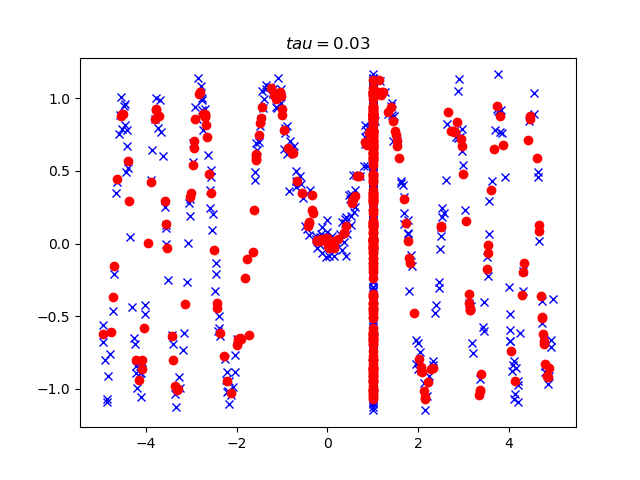
\includegraphics[width=\linewidth]{pics/tau_0d03}
    \end{subfigure}
    \begin{subfigure}[b]{0.5\linewidth}
        \centering
        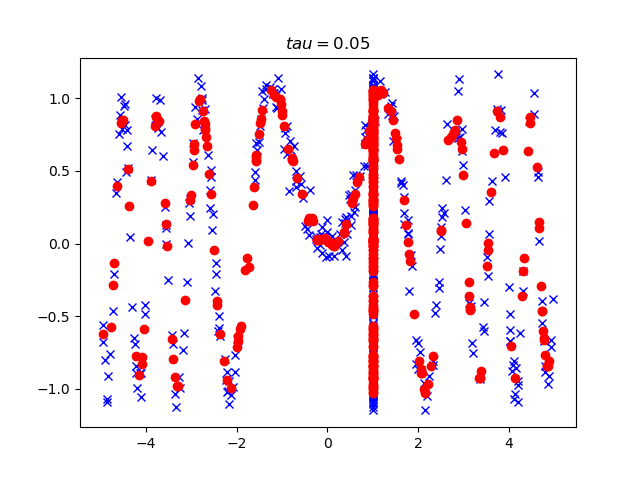
\includegraphics[width=\linewidth]{pics/tau_0d05}
    \end{subfigure}
    \begin{subfigure}[b]{0.5\linewidth}
        \centering
        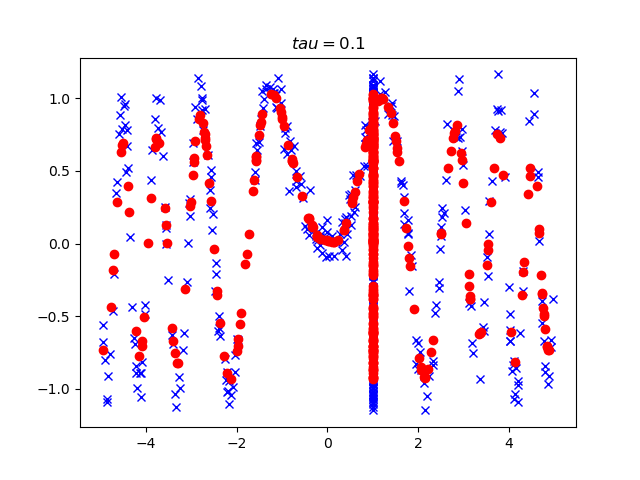
\includegraphics[width=\linewidth]{pics/tau_0d1}
    \end{subfigure}
    \begin{subfigure}[b]{0.5\linewidth}
        \centering
        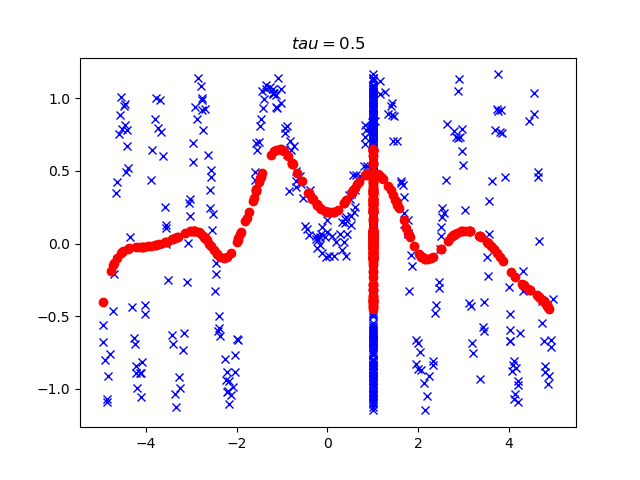
\includegraphics[width=\linewidth]{pics/tau_0d5}
    \end{subfigure}
    \begin{subfigure}[b]{0.5\linewidth}
        \centering
        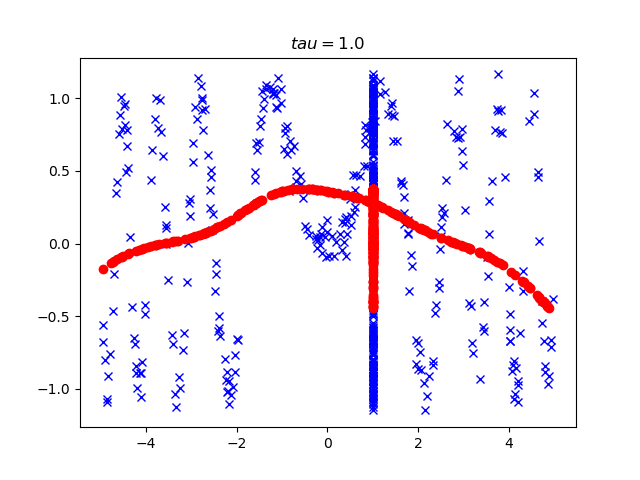
\includegraphics[width=\linewidth]{pics/tau_1d0}
    \end{subfigure}
    \begin{subfigure}[b]{0.5\linewidth}
        \centering
        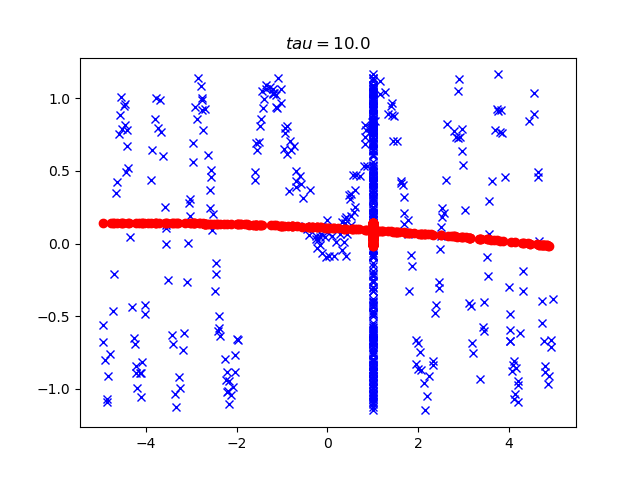
\includegraphics[width=\linewidth]{pics/tau_10d0}
    \end{subfigure}

$tau = 0.05$ achieve best result. MSE on valid set is $0.0124$, on test set is $0.0170$.

\end{figure}
\end{answer}

} \fi

\end{enumerate}


\end{enumerate}

\end{document}
